\section{Resultados}

\subsection{Entorno de ejecución}
Los algoritmos se implementaron en Python con NumPy y SciPy \cite{scipy20}. El solver exacto es HiGHS \cite{highs18} con un límite de tiempo de 600 segundos. El Algoritmo Genético se ejecutó con semillas distintas para cada corrida. Los tiempos de cómputo dependen del equipo en que se ejecuta el código, por lo que deben leerse como una comparación relativa entre métodos y no como valores absolutos.

\subsection{Solución exacta}
El solver HiGHS no logró demostrar la optimalidad en los 600 segundos permitidos. Terminó con la mejor solución entera encontrada, de \textbf{costo 50\,119} y 22 antenas, una cota inferior (\textit{dual bound}) de 30\,817 y una brecha de optimalidad de 38,5\,\%. Exploró 19\,036 nodos del árbol de ramificación. La relajación lineal del modelo, que se resuelve en menos de un segundo, da una cota inferior de 27\,860. Es decir, el costo óptimo está entre 30\,817 y 50\,119, según lo que el solver pudo demostrar.

Este comportamiento es el esperado para una instancia densa de $500\times500$: cada cliente tiene entre 32 y 70 antenas que lo cubren, de modo que hay muchísimas combinaciones casi equivalentes y la cota inferior mejora muy lentamente, como lo discuten Caprara, Fischetti y Toth \cite{caprara00}.

\subsection{Heurística voraz de referencia}
Como referencia adicional se aplicó la heurística voraz de Chv\'atal \cite{chvatal79}, que es la fase de cobertura de la reparación del Algoritmo Genético. Obtuvo un costo de 52\,063 con 23 antenas en menos de 0,01 segundos.

\subsection{Algoritmo Genético}
La Tabla~\ref{tab:ga} resume 10 corridas independientes por configuración. La configuración \textit{extendida} usa población de 200, mutación $2/n$, hasta 3\,000 generaciones y paciencia de 400 generaciones.

\begin{table}[H]
\centering
\caption{Resultados del Algoritmo Genético (10 corridas por configuración). La brecha se mide contra la mejor solución entera del solver exacto (50\,119); un valor negativo significa que el AG obtuvo menor costo.}
\label{tab:ga}
\small
\begin{tabular}{lrrrrrrr}
\toprule
Configuración & Mejor & Media & Desv. & Peor & Tiempo (s) & Brecha mejor & Brecha media\\
\midrule
Base ($N=100$, $p_m=1/n$) & 48\,878 & 51\,622 & 1\,500 & 53\,807 & 2,1 & $-2{,}5\,\%$ & $+3{,}0\,\%$\\
Población pequeña ($N=30$) & 50\,914 & 54\,134 & 1\,712 & 57\,351 & 0,7 & $+1{,}6\,\%$ & $+8{,}0\,\%$\\
Población grande ($N=300$) & 49\,774 & 50\,809 & 992 & 53\,414 & 7,3 & $-0{,}7\,\%$ & $+1{,}4\,\%$\\
Mutación alta ($p_m=5/n$) & 49\,678 & 51\,452 & 1\,328 & 53\,976 & 3,1 & $-0{,}9\,\%$ & $+2{,}7\,\%$\\
Extendida ($N=200$, $p_m=2/n$) & 49\,678 & 50\,436 & 606 & 52\,038 & 16,6 & $-0{,}9\,\%$ & $+0{,}6\,\%$\\
\bottomrule
\end{tabular}
\end{table}

\begin{figure}[H]
\centering
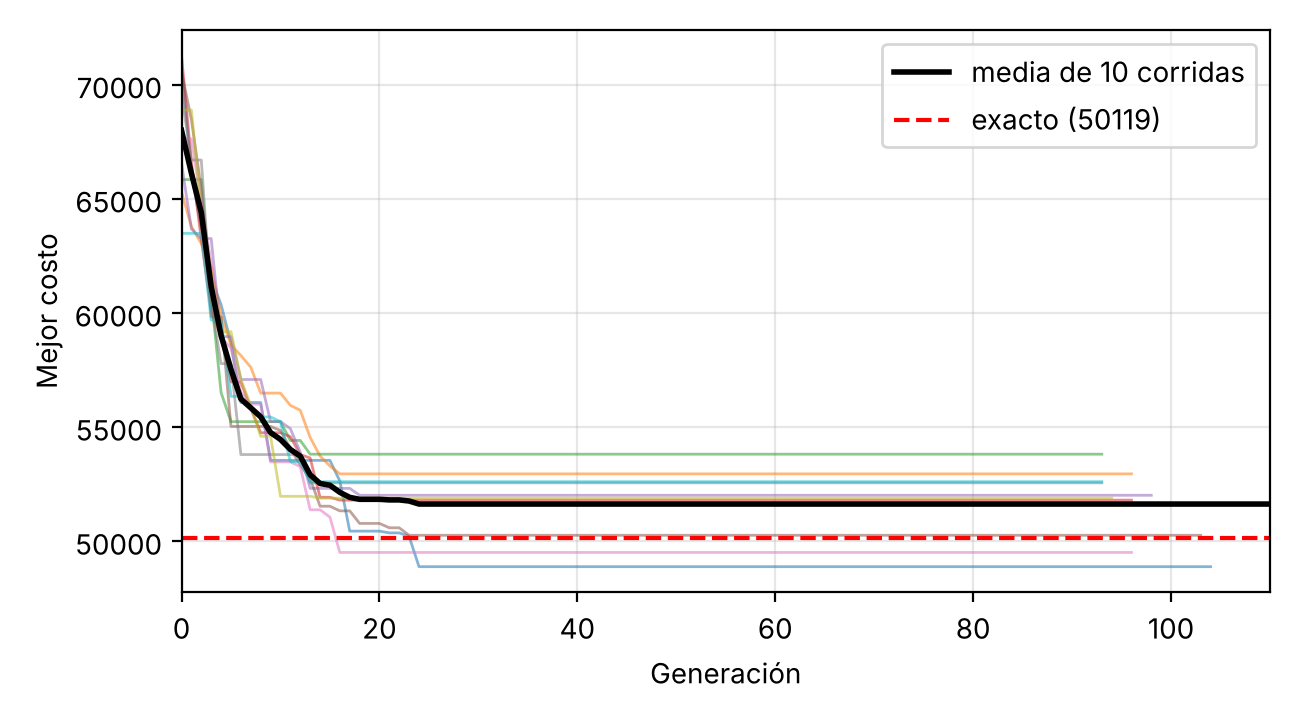
\includegraphics[width=0.85\textwidth]{figuras/convergencia.png}
\caption{Convergencia del Algoritmo Genético (configuración base). Las líneas delgadas son las 10 corridas; la línea gruesa es su promedio; la línea roja punteada es el costo de la mejor solución del solver exacto.}
\label{fig:conv}
\end{figure}

La Figura~\ref{fig:conv} muestra que el AG mejora rápidamente en las primeras 20 a 25 generaciones, partiendo de costos cercanos a 68\,000, y después se estanca: la mayoría de las corridas deja de mejorar y se detiene por el criterio de paciencia hacia la generación 100. Esto indica convergencia prematura: la población pierde diversidad y el cruce deja de producir mejoras.

\begin{figure}[H]
\centering
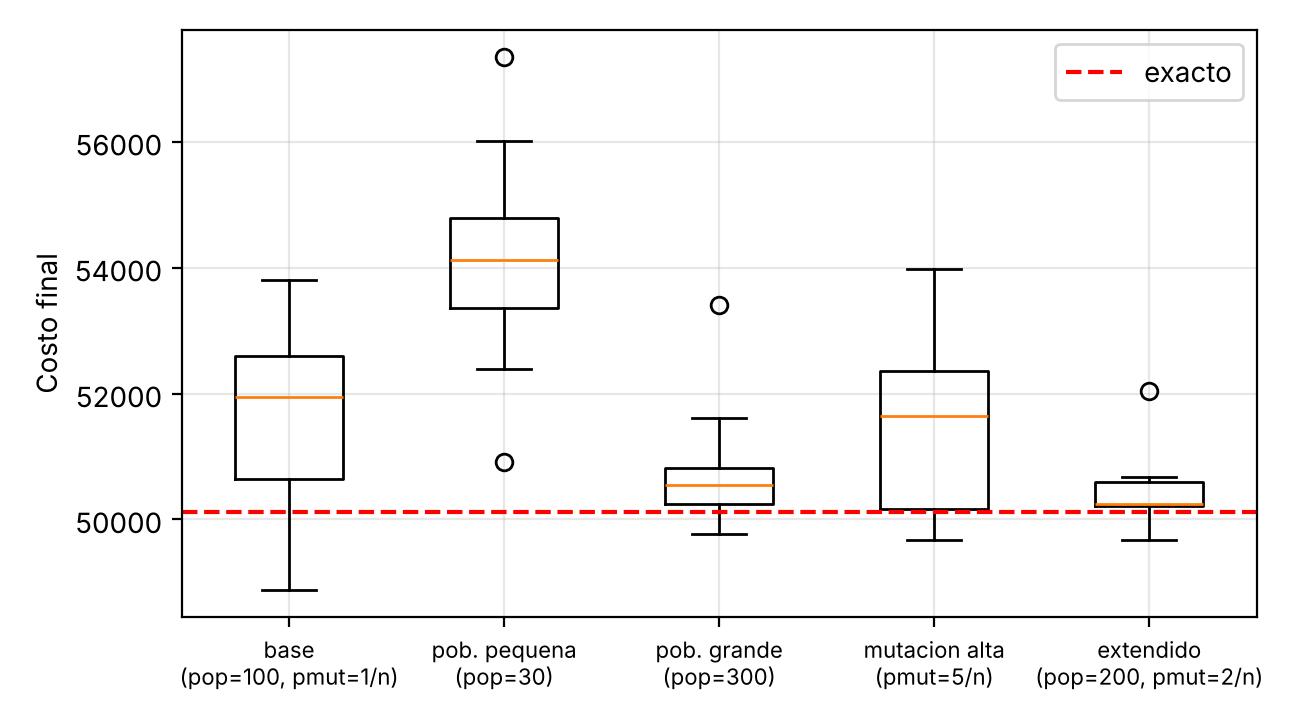
\includegraphics[width=0.85\textwidth]{figuras/boxplot_config.png}
\caption{Distribución del costo final por configuración del AG (10 corridas cada una). La línea roja es la mejor solución del solver exacto.}
\label{fig:box}
\end{figure}

\subsection{Comparación entre el método exacto y el Algoritmo Genético}
La Figura~\ref{fig:comp} compara los costos de todos los métodos y la Tabla~\ref{tab:comp} los resume junto con sus tiempos.

\begin{figure}[H]
\centering
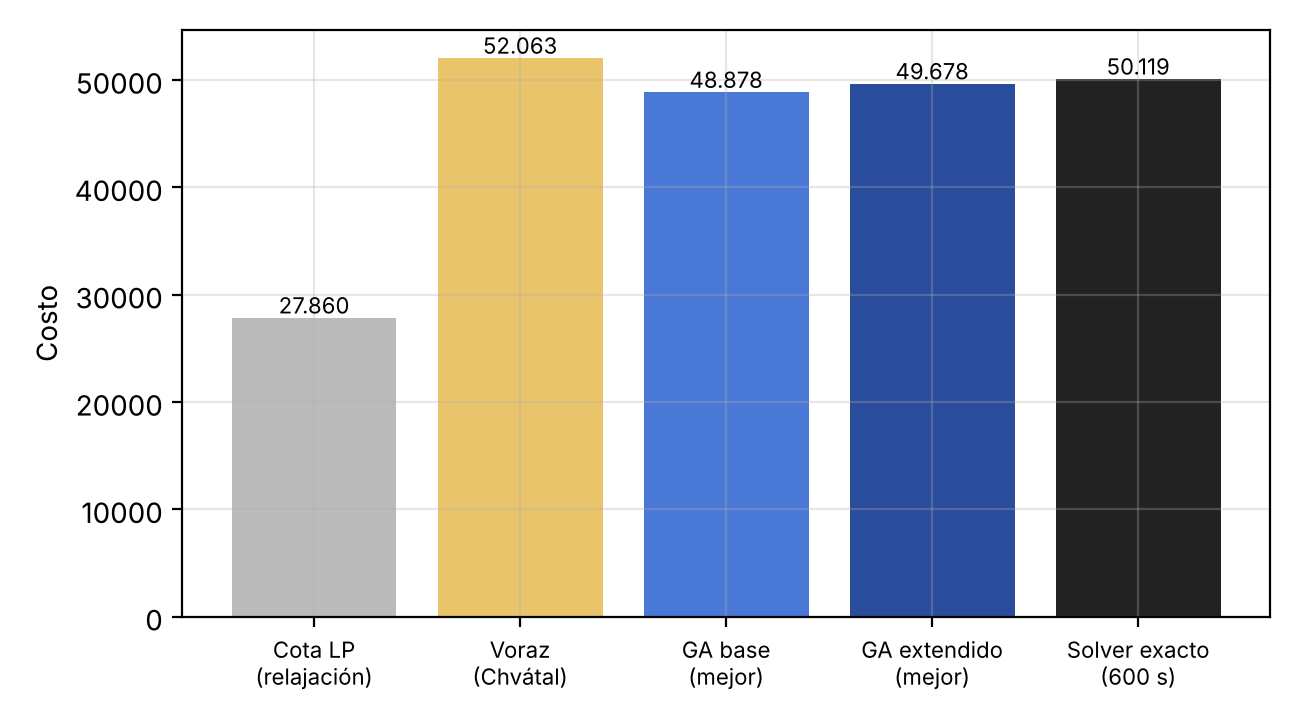
\includegraphics[width=0.85\textwidth]{figuras/comparacion.png}
\caption{Costo obtenido por cada método.}
\label{fig:comp}
\end{figure}

\begin{table}[H]
\centering
\caption{Comparación de métodos.}
\label{tab:comp}
\begin{tabular}{lrrr}
\toprule
Método & Costo & Antenas & Tiempo (s)\\
\midrule
Cota inferior (relajación lineal) & 27\,860 & -- & 0,2\\
Cota inferior del solver (600 s) & 30\,817 & -- & 600\\
Solver exacto (mejor entera) & 50\,119 & 22 & 600\\
Heurística voraz & 52\,063 & 23 & $<0{,}01$\\
AG base (mejor de 10) & 48\,878 & -- & 2,1 (promedio)\\
AG base (media de 10) & 51\,622 & 23,6 & 2,1\\
AG extendido (media de 10) & 50\,436 & 23,0 & 16,6\\
\bottomrule
\end{tabular}
\end{table}

\begin{figure}[H]
\centering
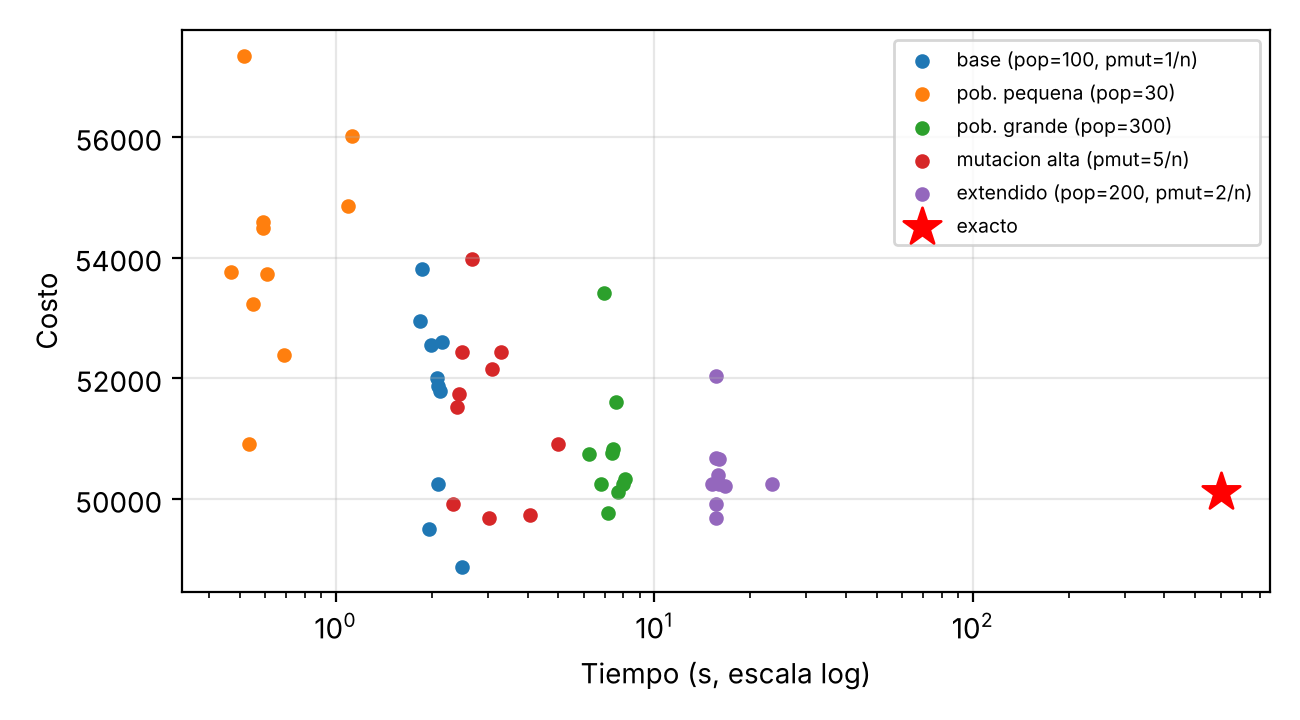
\includegraphics[width=0.85\textwidth]{figuras/costo_vs_tiempo.png}
\caption{Costo frente al tiempo de cómputo (escala logarítmica en el tiempo). La estrella roja es el solver exacto.}
\label{fig:tiempo}
\end{figure}

\subsection{Análisis}
\textbf{Calidad de la solución.} La mejor solución encontrada por el AG (48\,878, en la configuración base) es 2,5\,\% más barata que la mejor solución entera que el solver encontró en 600 segundos, y 6,1\,\% más barata que la heurística voraz. Sin embargo, el AG es estocástico: en la configuración base el costo medio es 3,0\,\% mayor que el del solver y varía entre 48\,878 y 53\,807. La configuración extendida es más estable (desviación de 606) y su media queda a 0,6\,\% del solver.

\textbf{Tiempo de cómputo.} El AG base necesita unos 2 segundos por corrida; el solver agotó 600 segundos sin demostrar optimalidad. El AG llega a soluciones de calidad comparable en una fracción del tiempo.

\textbf{Efecto de los parámetros.} Una población pequeña ($N=30$) empeora claramente los resultados (media $+8{,}0\,\%$ sobre el solver) porque explora poco. Una población mayor reduce la media y la dispersión, pero cuesta más tiempo (7,3\,s con $N=300$). Aumentar la mutación a $5/n$ mejora levemente el mejor resultado sin costo de tiempo importante. La configuración extendida logra la mejor media y la menor dispersión al precio de unos 17 segundos.

\textbf{¿El AG alcanzó el óptimo?} No se puede afirmar. El solver no demostró la optimalidad, y su mejor cota inferior es 30\,817, de modo que el costo óptimo está entre 30\,817 y 48\,878 (la mejor solución conocida). Lo que sí se puede afirmar es que el AG obtuvo soluciones factibles de menor costo que las del solver en el tiempo límite. Para saber qué tan lejos está del óptimo haría falta un solver con más tiempo o una cota inferior más fuerte.
